\chapter{Scalabilit\'a, Pro e Contro}\label{cap:scalprocont}
\section{Scalabilit\'a}\label{sez:scalabilita}
La Scalabilit\'a, ossia la capacit\'a dell'applicazione di resistere all'aumentare del numero di utenti concorrenti che ne usufruiscono, dipende fortemente dal modello scelto, come anche dalla tipologia di applicazione sviluppata.
Quindi scegliere il modello pi\'u adatto non \`e banale e non ne esiste uno standard sempre corretto.

Il problemi introdotti dalla scalabilit\'a comunque sono fondamentalmente diversi tra Blazor Server, e tutti gli altri modelli.
Questo principalmente per 3 motivi:
\begin{enumerate}
	\item Blazor Server delega completamente al server che ospita l'applicazione il carico computazionale necessario per gestire ogni singolo evento della UI di ogni sessione per ogni utente connesso, compreso il salvataggio in memoria RAM dello stato di ciascuna UI durante l'utilizzo dell'applicazione, visto che ad ogni browser coinvolto, dopo l'inizializzazione, arrivano solamente le minime differenze necessarie per effettuare il render della ui rispetto al frame precedente, ogni volta che deve cambiare qualcosa.
	Ci\`o implica che la potenza del server debba tener conto di eventuali picchi di utenze, e debba avere a disposizione sufficiente RAM per poter mantenere in memoria lo stato dell'applicazione di ciascun utente concorrente connesso.
	
	\item Il secondo \`e che Blazor Server, necessita di almeno una connessione costante ed affidabile con ogni sessione di ogni utente collegato.
	
	\item Il terzo \`e che questo modello sfrutta SignalR, che per funzionare al meglio utilizza il protocollo di trasporto WebSocket, quindi la macchina server sul quale viene ospitata l'applicazione Blazor \`e consigliato che lo supporti, pur non essendo necessario.
\end{enumerate}

Gli altri modelli invece sfruttano l'hardware di ogni client connesso, come solitamente avviene per le SPA odierne.
Sono quindi in linea con il comportamento degli altri framework basati su Javascript come i gi\'a citati Angular React o Vue.js, in particolare Blazor WebAssembly. 
Di seguito verranno quindi confrontati pro e contro dell'utilizzo del modello Blazor Server e del modello Blazor WebAssembly, partendo dai punti evidenziati nella figura \ref{fig:blazorModelsProCons}.
\begin{figure}[H]
	\centerline{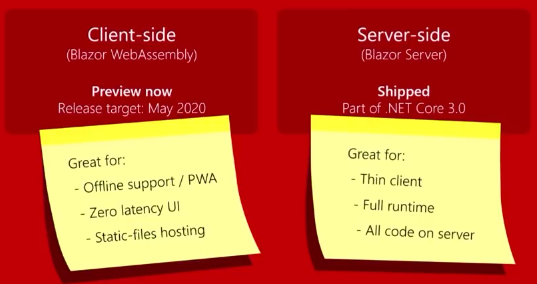
\includegraphics[scale=0.8]{figure/ClientServerProCons.png}}
	\caption{Confronto Modelli Client-Server}
	\label{fig:blazorModelsProCons}
\end{figure}

\section{Quando usare Blazor Server}\label{sez:scalabilitaBServer}
\subsection{Pro}\label{sez:proBServer}
Questo modello vanta, come primo punto a favore, il fatto di essere stato creato per essere una soluzione completa, ma che pu\`o essere utilizzata in modo complementare in applicazioni gi\'a esistenti che ad esempio si basano su Razor.
Si pu\`o quindi andare ad ampliare queste applicazioni senza doverle riscrivere da zero.
In questo modo si possono continuare a sfruttare le pagine completamente renderizzate lato server dove necessario, ma si possono anche gestire le interazioni del client con la UI potendo referenziare codice C\# senza doverlo riscrivere in Javascript o anche solo passare tramite JS, in parti dell'applicazione dove si ritiene sia pi\'u adatto farlo.

Un altro grande pro di questo modello \`e il fatto di poter delegare al server la responsabilit\'a di dover sopportare un peso maggiore, al crescere dell'applicazione, mentre il client non deve scaricare pi\'u dati.
Infatti i file scaricati lato client sono solo quelli necessari all'inizializzazione della UI e allo stabilimento di una connessione con il server, che quindi al crescere del peso dell'applicazione, non invia dati in pi\'u ai client, ma continua solamente a inviare le differenze della UI rispetto allo stato precedente.
Questo secondo vantaggio, rende il modello ideale per i casi in cui si deve creare un'applicazione per nella quale i client che la utilizzeranno potrebbero avere a disposizione computer o cellulari a basso costo.

Il terzo punto a favore, molto utile durante lo sviluppo di applicazioni \`e che il codice dinamico relativo alla logica dell'applicazione sviluppata, comprese eventuali logiche di business, non escono mai dal server, in quanto tutto viene eseguito lato server dopo la connessione iniziale.

Il quarto punto a favore, \`e che se si vuole sviluppare un'applicazione Blazor da utilizzare in produzione, fino a maggio 2020 questo modello \`e l'unico ad essere ufficialmente supportato e che si pu\`o quindi cominciare gi\'a ad utilizzare.

Infine il fatto che l'applicazione esegua sul server, implica che si possa utilizzare l'intero runtime di .NET Core, che implementa completamente il .NET Standard 2.0.
\subsection{Contro}\label{sez:controBServer}
Il principale punto a sfavore di questo modello \`e la gi\'a citata RAM consumata da ogni UI per ogni sessione di ogni utente che utilizza l'applicazione.
Un benchmark eseguito da Microsoft a tal proposito, ha mostrato come il principale collo di bottiglia di una applicazione Blazor sia proprio la RAM.
Microsoft ha dichiarato che hanno stimato vengano occupati in media 250KB in RAM per ogni nuova connessione di un utente ad una applicazione base di tipo hello world e consigliano di dedicare almeno 273 KB per utente se non si ha chiaro da dove partire.Durante il test di carico svolto da Microsoft \`e stata utilizzata una sola macchina virtuale Azure di fascia medio-bassa(Standard D1V2)come server per ospitare l'applicazione Blazor, avendo quindi a disposizione 3.5 GB di RAM e le caratteristiche visibili in figura \ref{fig:vmStandardD1V2}.

\begin{figure}[H]
	\centerline{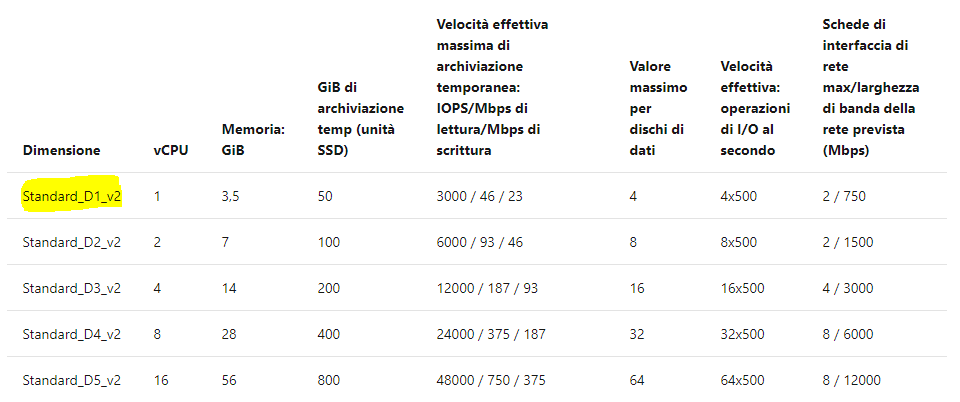
\includegraphics[scale=0.5]{figure/Standard_D1_V2.PNG}}
	\caption{Parametri VM utilizzata per il test di carico}
	\label{fig:vmStandardD1V2}
\end{figure}

Con questi parametri, l'applicazione \`e stata in grado di gestire 5000 utenti concorrenti senza perdita significativa di performance \cite{blazorModelsScenarios} \cite{bServerConcurrentUsersTest}.
Bisogna quindi tener conto che al crescere delle informazioni da tenere in memoria per ciascun utente, l'applicazione sviluppata richieder\'a pi\'u RAM per ciascuno, quindi per questo modello i costi dell'infrastruttura dipendono fortemente dai volumi di utenti concorrenti che la utilizzano.

\section{Quando usare Blazor WebAssembly}\label{sez:scalabilitaBWA}
\subsection{Pro}\label{sez:proBWA}


\subsection{Contro}\label{sez:controBWA}